\documentclass[tikz,border=2pt]{standalone}
\usepackage[T1]{fontenc}\usepackage[utf8]{inputenc}\usepackage{mathptmx}
\usepackage{pgfplots}\pgfplotsset{compat=1.18}
\pgfkeys{/pgf/number format/.cd,use comma,precision=2,fixed,fixed zerofill}
\definecolor{oscuro}{HTML}{4F7DB9}
\begin{document}
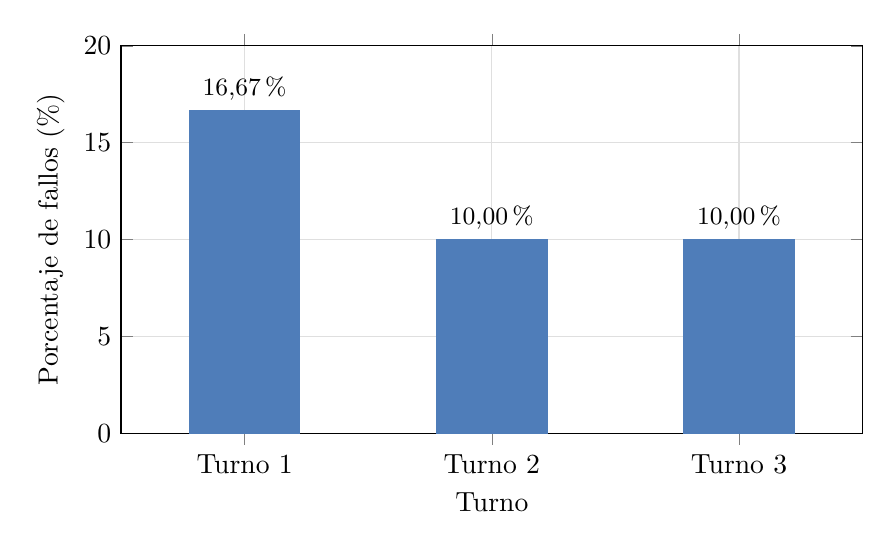
\begin{tikzpicture}
\begin{axis}[ybar, width=11cm, height=6.5cm, bar width=14mm, ymin=0, ymax=20,
  ylabel={Porcentaje de fallos (\%)}, xlabel={Turno}, symbolic x coords={Turno 1,Turno 2,Turno 3},
  xtick=data, enlarge x limits=0.25, ytick={0,5,10,15,20}, yticklabel={\pgfmathprintnumber[fixed,precision=0]{\tick}}, grid=major, grid style={gray!25},
  nodes near coords={\pgfmathprintnumber[fixed,precision=2,fixed zerofill]{\pgfplotspointmeta}\,\%},
  every node near coord/.append style={font=\small}, bar shift=0pt]
\addplot[fill=oscuro, draw=oscuro] coordinates {(Turno 1,16.67) (Turno 2,10.00) (Turno 3,10.00)};
\end{axis}
\end{tikzpicture}
\end{document}
